\begin{frame}{}
  \scriptsize
  Formez des groupes selon le type d'endroit (les 4 choix) où vous voudriez habiter.
  Tout le monde qui choisit une ville se regroupe, tout le monde qui choisit une banlieue se regroupe, etc.
  Discutez des raisons que vous avez choisi l'endroit, et faites une liste de ses avantages que vous allez présenter à la classe.
  \begin{center}
  \parbox{0.49\linewidth}{
    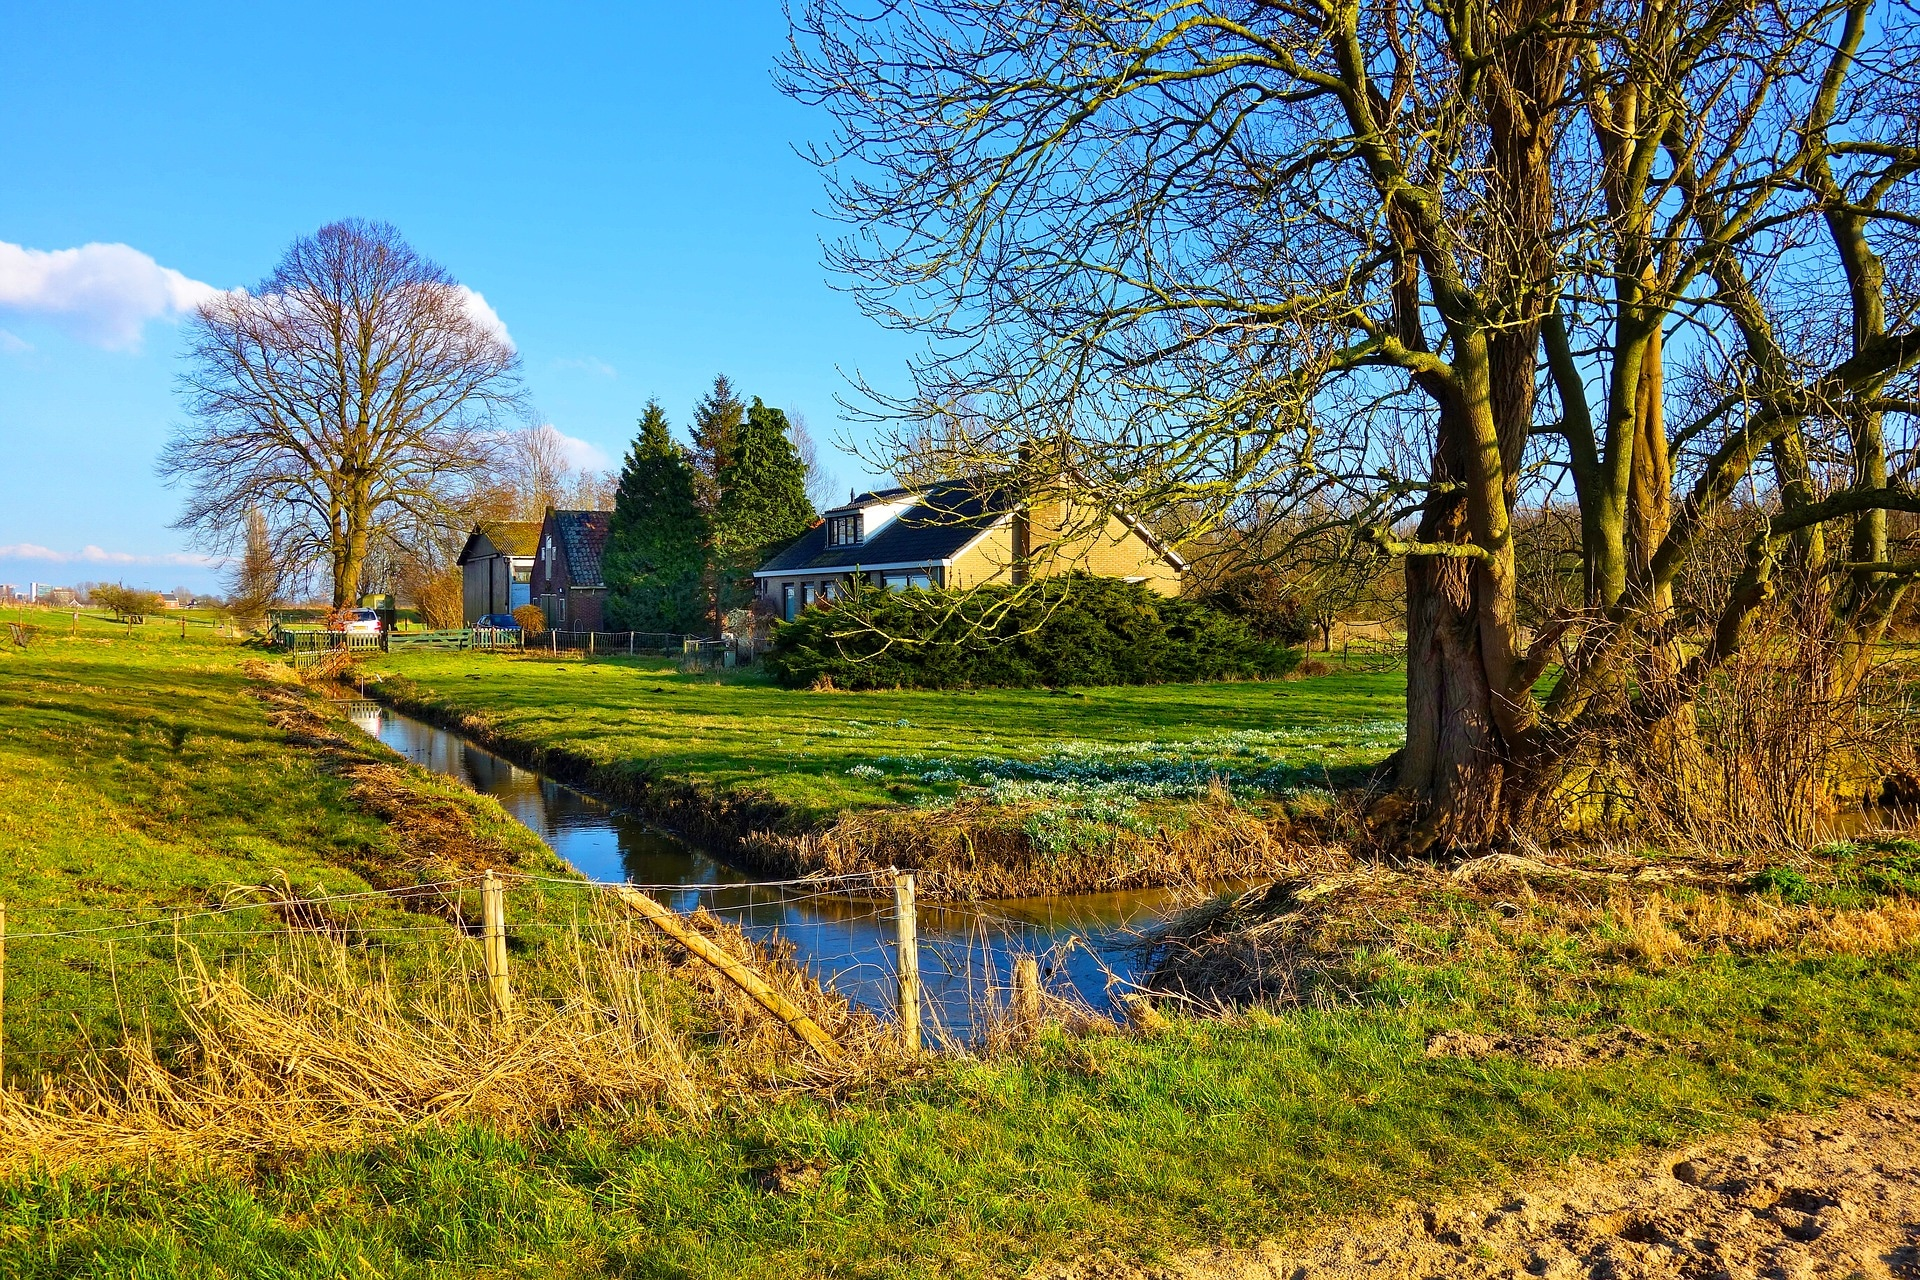
\includegraphics[scale=0.075]{campagne.jpg} \\
    la campagne
  }
  \parbox{0.49\linewidth}{
    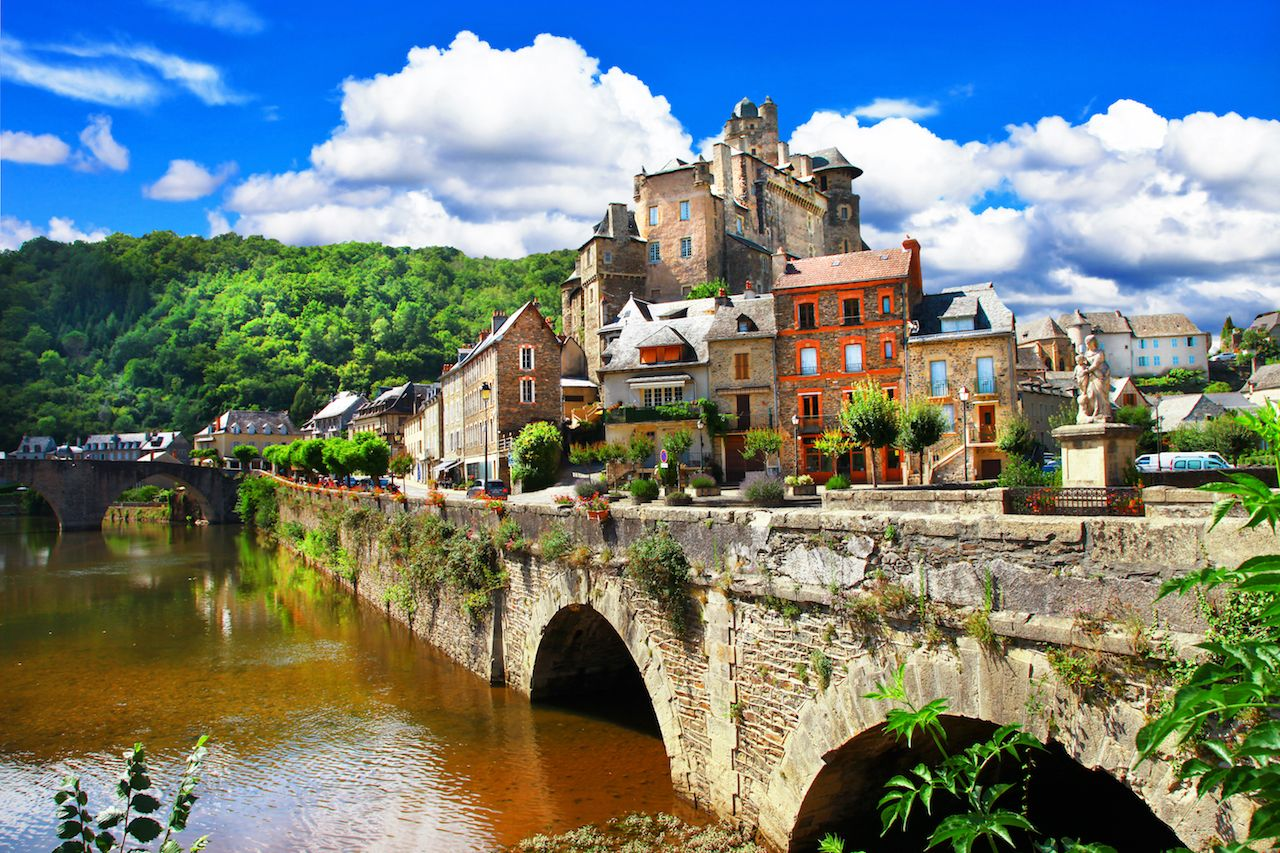
\includegraphics[scale=0.15]{estaing_france.jpg} \\
    un village (Estaing, France)
  } \\
  \parbox{0.49\linewidth}{
    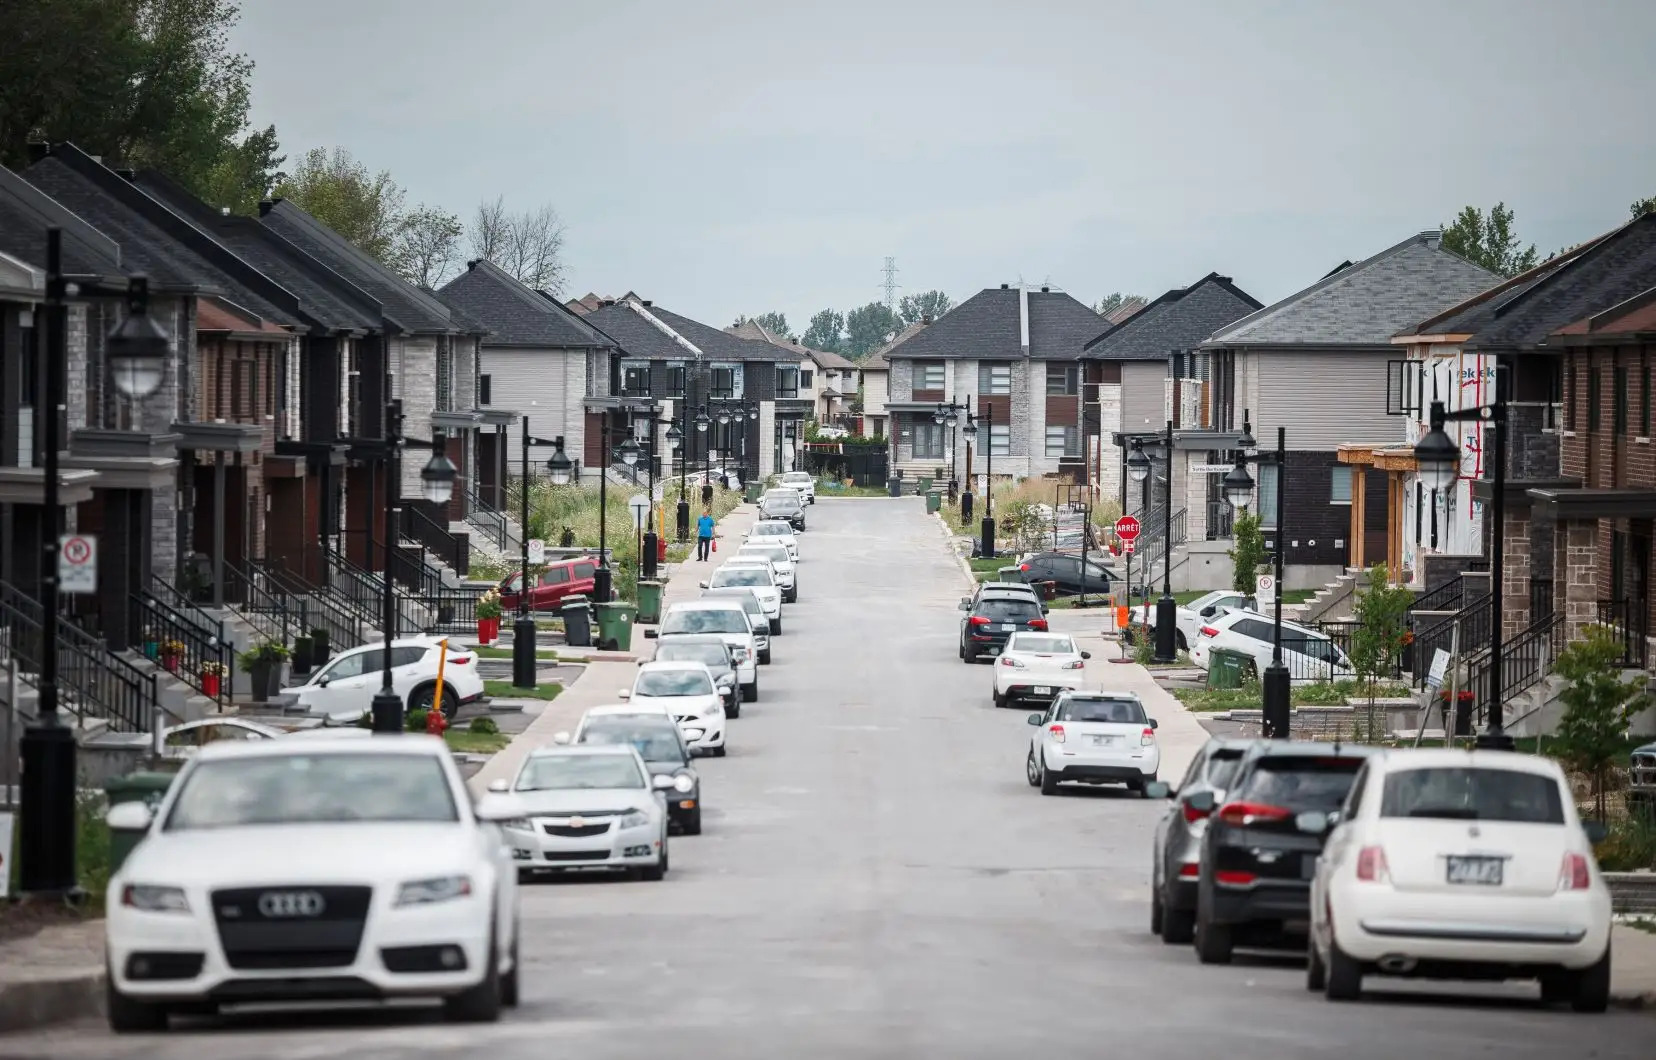
\includegraphics[scale=0.077]{banlieue_montreal.jpg} \\
    une banlieue (de Montréal)
  }
  \parbox{0.49\linewidth}{
    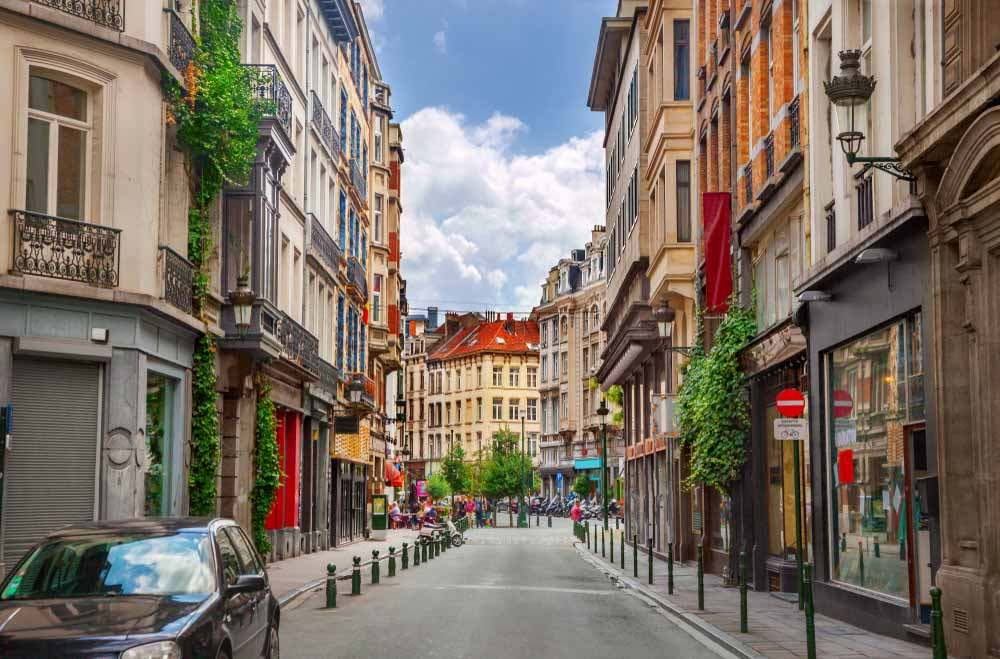
\includegraphics[scale=0.4]{bruxelles.jpg} \\
    une ville (Bruxelles)
  }
  \end{center}
\end{frame}